\documentclass[xcolor=dvipsnames]{beamer}

%\documentclass[pdf]{beamer}
\usetheme{Warsaw}
%\usepackage{color}
\usepackage[fleqn,tbtags]{mathtools,amsmath}
\usepackage{xcolor,minted,tikz,circuitikz}
%\usepackage{intersections, calc}
\setcounter{MaxMatrixCols}{13}
%\usepackage[dvipsnames]{xcolor}
\definecolor{UBCblue}{rgb}{0.04706, 0.13725, 0.26667} % UBC Blue (primary)

\definecolor{UBCblue}{rgb}{0.04706, 0.13725, 0.26667} % UBC Blue (primary)
\definecolor{UBCgrey}{rgb}{0.3686, 0.5255, 0.6235} % UBC Grey (secondary)

\setbeamercolor{palette primary}{bg=UBCblue,fg=white}
\setbeamercolor{palette secondary}{bg=UBCblue,fg=white}
\setbeamercolor{palette tertiary}{bg=UBCblue,fg=white}
\setbeamercolor{palette quaternary}{bg=UBCblue,fg=white}
\setbeamercolor{structure}{fg=UBCblue} % itemize, enumerate, etc
\setbeamercolor{section in toc}{fg=UBCblue} % TOC sections

% Override palette coloring with secondary
\setbeamercolor{subsection in head/foot}{bg=UBCgrey,fg=white}

%\newvector[A,\mathbf{A}]{A}


\newcommand{\dV}{\dot{V}}
\mode<presentation>{}
\title{Modelling District Heating and Cooling network}
\author{Leanne Dong}
\institute{Gina Cody School of Engineering and Computer Science\\ Concordia University Montr\'eal}
\begin{document}
%% title frame
\begin{frame}
\titlepage
\end{frame}
\begin{frame}{Overview}
\tableofcontents
\end{frame}


% \begin{frame}<presentation:0>{Road map}
% 	\begin{itemize}
% 	%	\item {\color{purple}Graph theory} and the topology to DHN
% 		\item {\color{purple}Hydraulic} Model: Mathematical Physical Modelling, numerical solution and optimization
% 		\item {\color{purple}Thermal} Model: Mathematical Physical Modelling, numerical solution and optimization
% 		\item {\color{purple}Hydraulic-Thermal} Model: Mathematical Physical Modelling, numerical solution and optimization
% 	\end{itemize}
% \end{frame}
%% normal frame
\section{Fundamentals}

\subsection{General concepts}
\begin{frame}{District Heating and Cooling Networks (DHN)}
\begin{itemize}
	\item The most common method for heating building in cities
	\item Usually consist of supply and return pipes that deliver heat in form of hot water or stream
\end{itemize}
\end{frame}

\subsection{Graph theory}

\begin{frame}{Common graph problems}
	\begin{itemize}
		\item Shortest Path Problem : Breadth First Search (BFS), Dijkstra's, Bellman-Ford, Floyd-Warshall
		\item {\color{red} Connectivity/Path finding: A* algorithm}, BFS, DFS
		\item Negative Cycle : Bellman-Ford, Floyd-Warshall
		\item Traveling Salesman Problem: 
		\item Bridges: These are edges in a graph whose removal could increase the number of connected components in the graph. They are important because they represent the vulnerabilities and bottlenecks with in the graph.
		\item Minimum Spanning Tree: Kruskal's and Prim's algorithm
		\item Maximum Network Flow: Ford-Fulkerson and Edmonds Karp\& Dinic's algorithms

	\end{itemize}
\end{frame}

\begin{frame}{Our graph problems}
	\textbf{Problem 1: }: Suppose there are 1000 building in a town, can we implement an algorithm that connects all the thousand building? Implement a A* algorithm.

	%Connectivity: nodes are given from the building location, footprint of the building needs to be known, we need to know the streets and green spaces, derive weighting factors between the connection possibilities depending on the cost of installing pipes under streets or on green spaces here is an extract from a commercial tool:Comsof Heat will automatically create a network topology which will connect each building to the network. Comsof Heat will divide the area into clusters, each supplied by a substation of a given power. Subsequently, the transport network will connect the source with the different substations. Streets and areas may be tagged with a reference cost. The automatic routing will avoid expensive streets and favour cheaper streets as much as possible. Furthermore, it is possible to classify the street cost based on the density of existing underground utilities. When maps with this information are available, the software can scan these files and create multiple categories with a different reference cost. The individual price per meter of the different types of pipe systems will be adjusted with the reference cost to come to an estimate with sufficient accuracy for a feasibility study.
\end{frame}

\begin{frame}
	The \textbf{Depth First Search (DFS)} is the most fundamental search algorithm used to explore nodes and edges of a 
	graph. It runs with a time complexity of $O(V+E)$ and is often used as a building block in other algorithms.

	By itself the DFS isn't all that useful, but when augmented to perform other tasks such as 
	\begin{itemize}
		\item Count connected components,
		\item Determine connectivity,
		\item Find bridges/articulation point.
	\end{itemize}
	then DFS really shines.
\end{frame}

\begin{frame}{General problems one may ask first}
Ask yourself:
	\begin{itemize}
		\item Is the graph directed or undirected?
		\item Are the edges of the graph weighted?
		\item Is the graph we will counter likely to be sparse or dense with edges?
		\item Should I use an adjacency matrix (or incidence matrix), adjacency list, an edge list or other structure to represent the graph efficiently?
	\end{itemize}
\end{frame}

%\subsection{Solution of linear systems}



% \subsection{Control theory}

% \begin{frame}{Background}
% 	Please refer to LC Evans control theory course \url{https://math.berkeley.edu/~evans/control.course.pdf}
% \end{frame}

% \begin{frame}{Problem}
% 	Control problem: (1) how do you adjust the flow rate in individual substations to that the return temperature has a given value (for example always 40°C)?
% \end{frame}

\section{Hydraulic Calculation}

\begin{frame}{Network graph}
	 	\begin{figure}[!ht]
  			\centering
    		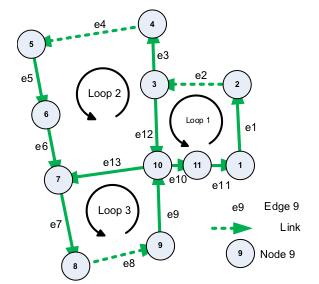
\includegraphics[width=5.5cm,height=5.5cm]{networkg.png}
    		 \caption[figure 3]{Network graph of the DH network in Scharnhauser Park}
    	\end{figure}
\end{frame}

\subsection{Numerical Solution}


\begin{frame}{Assumption}
\begin{itemize}
	\item 	The basic assumption for the calculation is incompressible media.
	\item 	Computation of flow distributions in DHN are mainly based on the Kirchhoff law for {\color{red}current} and {\color{blue}voltage} in circuits: The two equations describe {\color{red}flow rate} and {\color{blue}pressure losses} in the network
	\item 	Consider the PDE describing an one dimensional flow through a horizontal pipe which can be systematically derived from the Navier-Stokes equations.
\begin{align}
	\frac{l}{A}\frac{d\dot{m}}{dt}+\Delta p+R|\dot{m}|\dot{m}=0
\end{align}
Note: $\Delta p$ denoting the difference in pressure head between the two pipes ends and $\dot{m}$ is the mass flow rate. The variable $R$ stands for the hydraulic resistance of the pipe element, which is postulated to be a function of the physical properties such as length, roughness and diameter.
\end{itemize}
\end{frame}

\begin{frame}{Analogy of rules}
	\begin{table}[h!]
		\begin{center}
			\tikz\node[draw=red,thick,double,inner sep=1pt]{
			\begin{tabular}{p{15mm}|p{15mm}|p{15mm}|p{15mm}}
				\hline
				Electrical \newline network & Kirchoff's current \newline law & Kirchoff's voltage \newline law & Ohm's Law\\
				\hline
				District heating \newline network & Continuity of flow & Loop pressure \newline equations & Head loss \newline equations\\
			\end{tabular}};
		\end{center}
	\end{table}
\end{frame}

\begin{frame}{Contuinity of flow/Convervation of Mass}
The total amount of mass flow enter into a node is equal to the mass flow that leave the node plus the flow consumption at the node.
\begin{align}
		\sum \dot{V}_{\text{in}}-\sum \dot{V}_{\text{out}} = \dot{V}_{\text{mass}}
\end{align}
Assuming flow consumption is zero, 
\begin{align}
	\sum \dot{V}_{\text{in}}-\sum \dot{V}_{\text{out}} = 0
\end{align}
More concretely, 
\begin{align}\label{eq1}
	A\dot{V}=0
\end{align}
with the edge flow vector $\dV=\{\dV_1,\dV_2,\dV_z\}$, where $z$ is the number of edges.
\end{frame}

\begin{frame}[fragile,shrink=30]{Example: Benhassin\& Eicker 2013}
\begin{equation*}
	A = 
\begin{pmatrix*}
1 & 0 & 0 & 0 & 0 & 0 & 0 & 0 & 0 & 0 & -1 & 0 & 0\\
-1 & 1 & 0 & 0 & 0 & 0 & 0 & 0 & 0 & 0 & 0  & 0 & 0\\
0 & -1 & 1 & 0 & 0 & 0 & 0 & 0 & 0 & 0 & 0 & 0 & 0\\
0 & 0 & -1 & 1 & 0 & 0 & 0 & 0 & 0 & 0 & 0 & 0 & 0\\
0 & 0 & 0 & -1 & 1 & 0 & 0 & 0 & 0 & 0 & 0 & 0 & 0\\
0 & 0 & 0 & 0 & -1 & 1 & 0 & 0 & 0 & 0 & 0 & 0 & 0\\
0 & 0 & 0 & 0 & 0 & -1 & 1 & 0 & 0 & 0 & 0 & 0 &-1\\
0 & 0 & 0 & 0 & 0 & 0 & -1 & 1 & 0 & 0 & 0 & 0 & 0\\
0 & 0 & 0 & 0 & 0 & 0 & 0 & -1 & 1 & 0 & 0 & 0 & 0\\
0 & 0 & 0 & 0 & 0 & 0 & 0 & 0 & -1 & 1 & 0 & -1 & 1\\
0 & 0 & 0 & 0 & 0 & 0 & 0 & 0 & 0 & -1 & 1 & 0 & 0
\end{pmatrix*}
\end{equation*}

\begin{align*}
	B =
\begin{pmatrix}
	1 & 1 & 0 & 0 & 0 & 0 & 0 & 0 & 0 & 1 & 1 & 1 & 0\\
	0 & 0 & 1 & 1 & 1 & 1 & 0 & 0 & 0 & 0 & 0 & -1 & -1\\
	0 & 0 & 0 & 0 & 0 & 0 & 1 & 1 & 1 & 0 & 0 & 0 & 1
\end{pmatrix}
\end{align*}

Matrix $A$ is the incidence matrix that joins the nodes and the adjacent edges. \\

Matrix $B$ is a row for every loop and a column for every edge.
\end{frame}

\begin{frame}{Example: Benhassin\& Eicker 2013}
	For node 1, the conservation of mass is stated as 
	\begin{align*}
	 	\dV_1-\dV_{11}=0
	 \end{align*} 
	 or
	 \begin{align*}
	 	A\dV = 0
	 \end{align*}
\end{frame}

\begin{frame}{Loop pressure equations}
By the \textbf{conservation of energy}, the vector of loop pressure residual equals to 0
	\begin{align}\label{eq2}
	\Delta P = 0 
	\end{align}

That is, at each loop,
\begin{align}
\sum^{13}_{i=1}\Delta p_i = 0
\end{align}
In each loop, the pressure losses residual is composed of the pipe pressure losses in the same loop. In other words,
\begin{align}\label{eq3}
	\Delta P = B \Delta p
\end{align}
Hence we have 
\begin{align}\label{eq4}
	B\Delta p = \vec{0}
\end{align}
Note, the connecting branch currents are independent of each other, as they belong to different meshes. The column
of $B$-matrix indicate which connection branch current flow through the individual branches. That is,
\begin{align*}
\mathbf{B}&=B_{ij}
	= \begin{cases}
		1\quad \text{if flow in a pipe is the same direction as the definition}\\
		-1\quad \text{if flow in a pipe is the opposite direction as the definition}\\
		0\quad \text{if a pipe is not part of the loop}
	\end{cases}
\end{align*}
 The total current of a branch results as 
a linear superposition of these independent currents. More simply,
\begin{align}\label{eq5}
	\dV = B^T \dV_L
\end{align}
where $\dV=\{\dV_1, \dV_2, \dV_3\}.$ The equation dramatically reduces the number of unknown entities required to just three!
\end{frame}

\begin{frame}[fragile,shrink=30]{Loop pressure equations}
	Each pipe is considered as a flow resistance whose pressure is proportional to the square of its flow rate. That is,
	\begin{align}\label{eq6}
		\Delta p = K \dV^2
	\end{align}
where $K$ is the vector of resistance coefficient of each pipe given by the Darcy-Weisbech equation.

For every pipe, one gets
\begin{align}\label{eq7}
	\Delta p = f(\dV)
\end{align}
Hence (\ref{eq4}) becomes
\begin{align}\label{eq8}
	B\cdot f(\dV)=0
\end{align}
Substitute (\ref{eq5}) into (\ref{eq8}) we obtain:
\begin{align}
	B\cdot f(B^T\cdot \dV_L)=0
\end{align}
Apply the vector function
\begin{align}\label{eq10}
	F=f*B^T
\end{align}
Equation (\ref{eq10}) can be written as
\begin{align}\label{eq11}
	F(\dV_L)=0
\end{align}
The system of nonlinear equation (\ref{eq11}) can be solved via using Newton Raphson algorithm in following steps. 
First, we must define $F(\dV_L)$ and the Jacobien $DF$.
\end{frame}

\subsubsection{Solution of nonlinear systems}

\begin{frame}[shrink=20]{Nonlinear system and root finding}

\begin{itemize}
	%\item  $f$ is nonlinear when it fails the superposition principle: $f(x_1+x_2+\cdots)\neq f(x_1)+f(x_2)+\cdots$.
	\item A system of nonlinear equation is a set of equations 
	\begin{align*}
		f_1(x_1,x_2,\cdot,x_n)&=0,\\
		f_2(x_1,x_2,\cdot,x_n)&=0,\\
		&\shortvdotswithin{=}
		f_n(x_1,x_2,\cdot,x_n)&=0.
	\end{align*}
%where $(x_1,x_2,\cdots, x_n)\in\mathbb{R}^n$ and each $f_i$ is a nonlinear real function, $i=1,2,\cdots,n$
	\item There are three type of nonlinear system in hydraulic model. The solutions are usually found via 
	\textbf{Newton-Raphson} or Hardy Cross Method.

	\item An example of nonlinear system from the DHN in Scharnhauser Park (Hassine and Eicker 2011)

	\begin{align*}
		x^2-2x-y+0.5=0\\
		x^2+4*y^2-y-4=0
	\end{align*}

	\item To find the solution (root), we would use the C++ Linear algebra library {\color{purple}Eigen}.  %Note, Eigen might not work for more complicated nonlinearity...
	Codes: \url{https://godbolt.org/z/9NPKAA}

\end{itemize}
\end{frame}

\begin{frame}{Newtons algorithm}

\begin{columns}
	\begin{column}{.55\textwidth}
		\begin{itemize}
		\item Scalar case
			\begin{enumerate}
				\item Input: $v_0$, tolerance, eps
				\item Repeat
				\[v_0 = v - f(v)/f'(v)\]
				until $v_n-v\le$eps
				\item Print $v_n$, which is the root.
			\end{enumerate}
		\end{itemize}
	\end{column}
	\begin{column}{.75\textwidth}
 		\begin{itemize}
		\item Vector case
			\begin{enumerate}
				\item Input: $V_0$, \textbf{tolerance}, \textbf{eps}
				\item Repeat
				\[V_0 = V - DF(V)^{-1} F(V)\]
				until $V_n-V\le$eps
				\item Print $V_n$, which is the root.
			\end{enumerate}
		\end{itemize}
    \end{column}
\end{columns}
\textbf{Newton iteration}:
\begin{align*}
 	V^{k+1}:= V^k - \underbrace{DF(V^k)^{-1}F(V^k)}_{\text{correction}},\qquad DF(V^k)\,\,\text{sufficiently regular}
 \end{align*} 

\end{frame}

\subsection{Simulation}

\begin{frame}
	We would follow the same method used in electrical case. See circuit.pdf.
\end{frame}
% \begin{frame}{Network Topology}
% The description of the heating network is based on graph theory. First we need to form the topological matrice which show the structure of the mesh in matrix form. (See circuit.pdf)

% \end{frame}
% \begin{frame}{Graph Theory}
% 	Recall, the graph theory consider a network to be a compose of
% 	\begin{itemize}
% 		\item Nodes (Vertice)
% 		\item Edges (Branches are edges of a spanning tree)
% 		\item Loops 
% 		\item Meshes: a loop of a planar graph with no other branches inside
% 		\item Tree: a graph that is connected but got no loops
% 		\item Spanning Tree
% 	\end{itemize}
% \end{frame}

% \begin{frame}{Solution of network equation system}
% later
% \end{frame}


% \section{Thermal model}

% \begin{frame}{Preliminary: Numerical solution of differential equations}
	
% \end{frame}

% \subsection{Thermal Calculation}

% \begin{frame}{Numerical solution via finite difference or finite elements}
% 	By the first law of thermodynamics, the variation of the enthalpy of one pipe element is modelled by the
% 	following hyperbolic PDE:

% 	\begin{align}
% 		\frac{\partial(mf)}{\partial t}=\dot{H}-\dot{H}(x+\Delta x)-d\dot{Q}_l
% 	\end{align}
% \end{frame}

% \begin{frame}{Numerical Solution of the heat transfer in a pipe}
	
% \end{frame}

% \begin{frame}{Numerical Solution of heat transfer in the network}
	
% \end{frame}

% % \begin{frame}{Model Validation}
% % 	later
% % \end{frame}

% \section{Hydraulic-Thermal Model}

% \subsection{Calculation}

% \begin{frame}{Network structure}
% 	to be added
% \end{frame}

% \begin{frame}{Calculations}
% 		to be added
% \end{frame}


\end{document}